\section{Logistic Regression (LR)} \label{sec:prob1}
In this section, we consider Logistic Regression (LR) for binary classification of several 2D datasets, and compare the effect of different model parameters and regularization.

\subsection{Part 1}
We used SGD to optimize the LR objective with $L_2$ regularization, according to the equation:
\begin{equation}
E_{LR}(w,w_0) = \sum\limits_{i}log(1+exp(-y_i(w^Tx_i+w_0))) + \lambda||w||^2_2
\end{equation}
The decision boundary is shown in~\cref{fig:1_1_decision} for the cases of no regularization and some regularization ($\lambda=[0, 1]$).
When $\lambda=0$, $w=[1.73, -0.34, 4.55]$, and training accuracy is 100\%.
When $\lambda=1$, $w=[0.03, 0.03, 0.32]$, and there are some misclassified training samples, but the size of the weight vector is much smaller.

As iteration number increases, the weight vector converges to the learned weight, and the change between iterations gets smaller, shown in~\cref{table_lr_1_1}.

\begin{table}[ht!]
\centering
\begin{tabular}{||c c c||}  
 \hline
 Iteration & $w_1$ & $w_2$  \\ [0.3ex] 
 \hline\hline
 1 & -0.0069498 & 0.00896533 \\ 
 \hline
 2 & 0.00249062 & 0.02189003 \\ 
 \hline
 ... & & \\
 \hline
 39,999 & -0.34175886 & 4.55454265 \\ 
 \hline
 40,000 & -0.34173718 & 4.55456526 \\ 
 \hline
\end{tabular}
\caption{Accuracy of LR on four datasets.}
\label{table_lr_1_1}
\end{table}

\begin{figure}
	\centering
	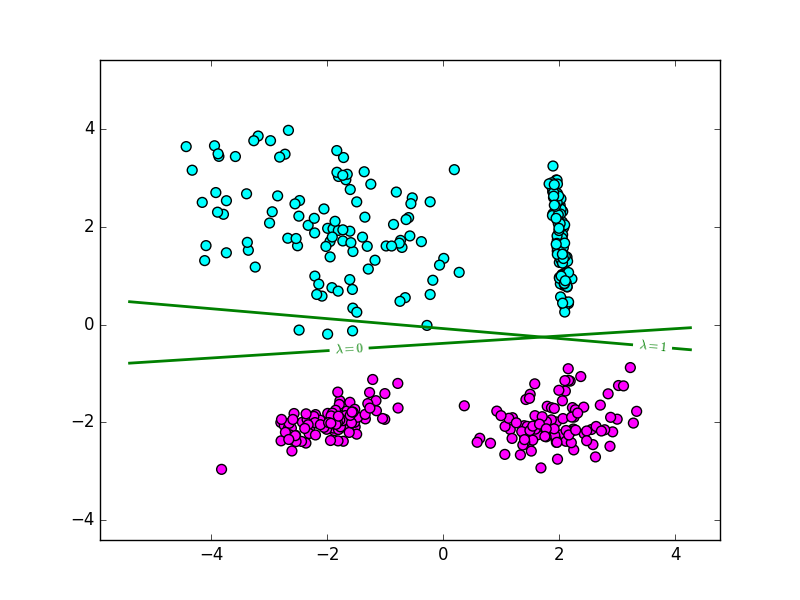
\includegraphics [trim=0 0 0 0, clip, angle=0, width=0.8\columnwidth,
	keepaspectratio]{figures/1_1_decision}
	\caption{LR decision boundaries for $L_2$ $\lambda=0$ and $\lambda=0$.}
	\label{fig:1_1_decision} 
\end{figure}

\subsection{Part 2}
An alternative regularization, $L_1$, was then compared against $L_2$ from the previous section.
In~\cref{fig:1_2_all_weights_good}, the elements of the weight vector are compared.
The top row shows $L_1$ regularization for each of the four datasets, and the bottom row shows $L_2$.
In general, increased regularization parameter, $\lambda$, causes smaller magnitude weight vector, since the blue and green points (small $\lambda$) are further from zero than the magenta and yellow points (large $\lambda$).
This is true for both $L_1$ and $L_2$ regularization.
Especially clear in the 2nd and 4th columns, $L_1$ regularization creates a more sparse weight vector, as all elements are zero (yellow) for the highly regularized case, whereas with the same regularization constant with a $L_2$ penalty has some non-zero elements.

In addition to the weight vector, the decision boundary is affected by $\lambda$ and regularization method.
In~\cref{fig:1_2_decision}, the decision boundaries for various $\lambda$ values are shown for same dataset with $L_1$ on the left and $L_2$ on the right.
As $\lambda$ increases, the boundary is placed in a position that will cause training errors ($\lambda > 1$).
The boundaries from the two regularization strategies are slightly different, but not by very much.
In~\cref{fig:1_2_decisions}, the same concept is shown across all four datasets, with the top row using $L_1$ and bottom row using $L_2$.
Green, blue, and yellow lines are decision boundaries with low $\lambda$, and red magenta, cyan are high $\lambda$.
Again, as $\lambda$ increases, training error increases. The first dataset (left) is linearly separable, the middle two have some class overlap, and the right dataset is not even close.
Accordingly, the decision boundary does not appear in the range of the data on the rightmost plot.

Finally, the test-set classification error is also compared across $\lambda$ values and regularization methods in~\cref{fig:1_2_accuracy}.
When $\lambda$ is very high for $L_1$ regularization (blue), test accuracy suffers, since model is too sparse.
$L_2$ reg. has almost constant accuracy throughout, but there is some small variation.
This is somewhat unexpected, because high regularization usually lowers model accuracy.
It could be that the effect is not seen in the range of $\lambda$'s shown.

\begin{figure}
	\centering
	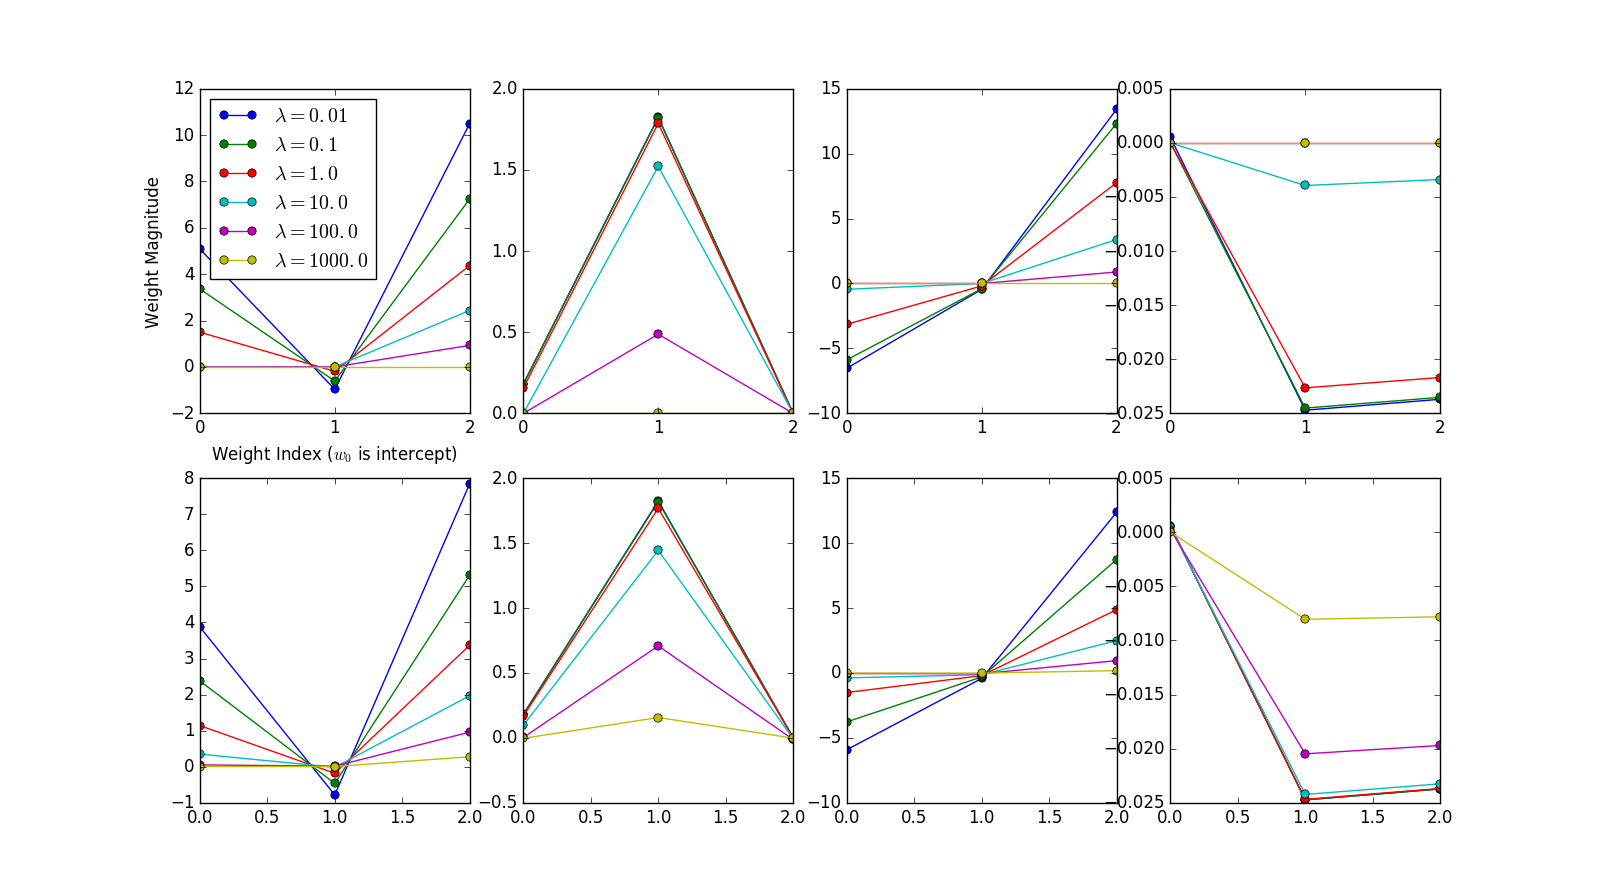
\includegraphics [trim=0 0 0 0, clip, angle=0, width=0.8\columnwidth,
	keepaspectratio]{figures/1_2_all_weights_good}
	\caption{Weight vectors of $L_1$ regularization (top row) and $L_2$ reg. (bottom row) for four datasets. Each column is the model for the same dataset. Within each subplot, several values of $\lambda$ are shown. For high lambda, weights are smaller in magnitude for all plots. $L_1$ reg causes sparser weight vector (more zero elements) than $L_2$.}
	\label{fig:1_2_all_weights_good} 
\end{figure}

\begin{figure}
	\centering
	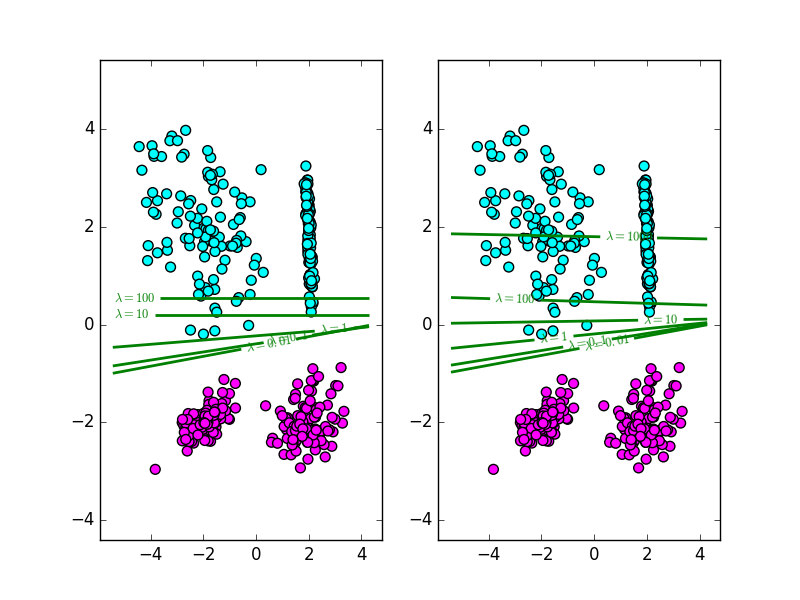
\includegraphics [trim=0 0 0 0, clip, angle=0, width=0.8\columnwidth,
	keepaspectratio]{figures/1_2_decision}
	\caption{LR on one dataset with $L_1$ reg on left, $L_2$ on right. Green lines show decision boundaries for various $\lambda$s. As $\lambda$ increases, training error increases.} 
	\label{fig:1_2_decision} 
\end{figure}

\begin{figure}
	\centering
	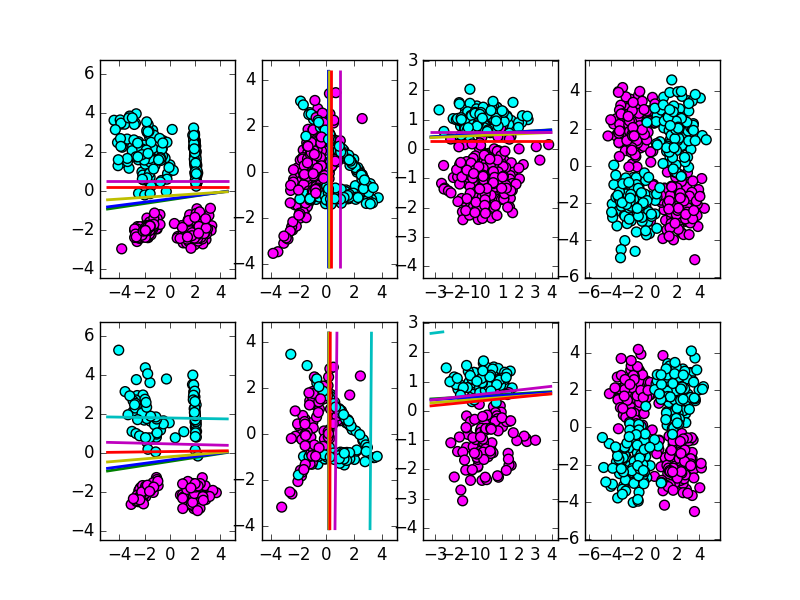
\includegraphics [trim=0 0 0 0, clip, angle=0, width=0.8\columnwidth,
	keepaspectratio]{figures/1_2_decisions}
	\caption{LR on four datasets, with the top row using $L_1$ and bottom row using $L_2$. Green, blue, and yellow lines are decision boundaries with low $\lambda$, and red magenta, cyan are high $\lambda$. As $\lambda$ increases, training error increases. The first dataset (left) is linearly separable, the middle two have some class overlap, and the right dataset is not even close. Accordingly, the decision boundary does not appear in the range of the data on the rightmost plot.} 
	\label{fig:1_2_decisions} 
\end{figure}

\begin{figure}
	\centering
	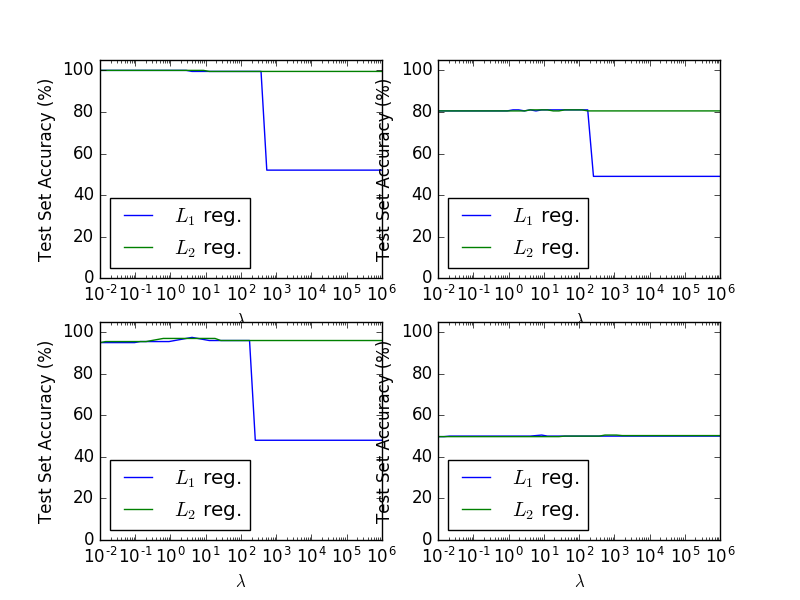
\includegraphics [trim=0 0 0 0, clip, angle=0, width=0.8\columnwidth,
	keepaspectratio]{figures/1_2_accuracy}
	\caption{For each dataset, the test accuracy is plotted across a wide range of $\lambda$ values. When $\lambda$ is very high for $L_1$ regularization (blue), test accuracy suffers, since model is too sparse. $L_2$ reg has almost constant accuracy throughout.} 
	\label{fig:1_2_accuracy} 
\end{figure}

\subsection{Part 3}
To pick the best regularizer and $\lambda$, the LR weights are trained with many values of $\lambda$ for each regularizer, using the training set.
Then, the generalization is evaluated on the validation set, by measuring the classification accuracy.
A model that generalizes well will have high accuracy on data not seen during training.
In cases where the validation accuracy is identical for multiple values of $\lambda$, the higher $\lambda$ is chosen, because this corresponds to lower model complexity (more regularized).
It is difficult to pick between $L_1$ and $L_2$ regularization because the boundaries aren't that different, as discussed earlier.
In case both validation accuracies are the same, $L_1$ may be slightly preferable to $L_2$ because of its sparsity.

\cref{table_lr_1_3} shows the accuracy of LR on the four datasets with optimized hyperparameters.
Training accuracy is greater than or equal to test accuracy for all datasets, as expected.
The accuracy numbers seem appropriate given the boundaries in~\cref{fig:1_2_decisions}: first and third columns are classified well by linear separator, second is decent, and fourth is not linearly separable in this feature space (the datasets are also described in later sections).


\begin{table}[ht!]
\centering
\begin{tabular}{||c c c c c||}  
 \hline
 Dataset & Regularizer & $\lambda$ & Train Acc. (\%) & Val. Acc. (\%) \\ [0.3ex] 
 \hline\hline
 1 & $L_2$ & 0.01 & 100.0 & 100.0 \\ 
 \hline
 2 & $L_2$ & 0.01 & 83.0 & 80.5 \\ 
 \hline
 3 & $L_1$ & 1.78 & 97.5 & 96.5 \\ 
 \hline
 4 & $L_2$ & 1000 & 51.75 & 50.5 \\ 
 \hline
\end{tabular}
\caption{Accuracy of LR on four datasets.}
\label{table_lr_1_3}
\end{table}
